\begin{pastexam}[label={px:ncu-115-dsa-18}]{中央資工所 115 學年度 第 18 題}
（複選；每題 5 分，全對才給分，答錯倒扣 1 分）

Given a binary tree with inorder traversal, \textbf{ILOVENCU}, and postorder traversal,
\textbf{LIVNUCEO}. Which of the following statements is (are) true?
\begin{enumerate}[label=\Alph*.]
\item The fifth letter in the level-order traversal is V.
\item The height of the binary tree is 5.
\item C is a leaf node.
\item The six letter in the level-order traversal is U.
\end{enumerate}
\end{pastexam}

\begin{pastsoln}
答案：A。

照資結書第~7.4~節的後序加中序重建：根是後序的最後一個，在中序裡切開，左子樹
有 $\ell$ 個節點時，後序的前 $\ell$ 個是左子樹。
\begin{center}
\begin{tabular}{llcll}
\toprule
子樹的後序 & 子樹的中序 & 根 & 左子樹（中序）& 右子樹（中序）\\
\midrule
LIVNUCEO & IL\,|\,O\,|\,VENCU & O & IL & VENCU \\
LI & |\,I\,|\,L & I & 空 & L \\
VNUCE & V\,|\,E\,|\,NCU & E & V & NCU \\
NUC & N\,|\,C\,|\,U & C & N & U \\
\bottomrule
\end{tabular}
\end{center}
樹是 $O\bigl(I(-, L),\; E(V, C(N, U))\bigr)$：
\begin{center}
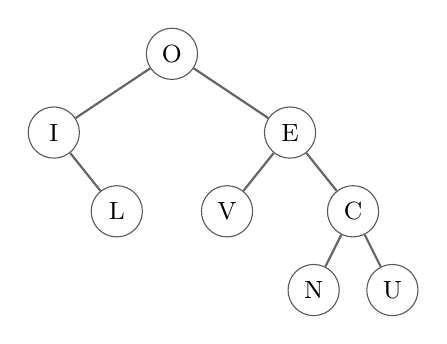
\begin{tikzpicture}[btn/.style={circle, draw=black!65, line width=0.4pt, minimum size=6.5mm, inner sep=0pt, font=\small}, level distance=10mm, edge from parent/.style={draw=black!60, thick}, level 1/.style={sibling distance=30mm}, level 2/.style={sibling distance=16mm}, level 3/.style={sibling distance=10mm}]
\node[btn] {O}
    child {node[btn] {I} child[missing] child {node[btn] {L}}}
    child {node[btn] {E}
        child {node[btn] {V}}
        child {node[btn] {C} child {node[btn] {N}} child {node[btn] {U}}}};
\end{tikzpicture}
\end{center}
驗算：這棵樹的中序是 ILOVENCU、後序是 LIVNUCEO，和題目相同。 層序是
$O\;I\;E\;L\;V\;C\;N\;U$。

\begin{itemize}
\item A 對。 層序第五個是 V。
\item B 錯。 這棵樹有 $4$ 層（$O$；$I, E$；$L, V, C$；$N, U$），照資結書的定義高度是
$4$，照數邊的定義是 $3$，兩種都不是 $5$。
\item C 錯。 $C$ 有兩個子節點 $N$、$U$，不是葉節點。
\item D 錯。 層序第六個是 C，U 是第八個。
\end{itemize}
\end{pastsoln}
